% Standalone section for the team's ICML file. Requires graphicx.
% Numbers come from output/idea5-language/summary.json (scripts/language_exploration.py).
% The discussion paragraph is provisional: replace it with your own reading before submission.
\section{Analysis: What the Language Modality Already Carries}
\paragraph{Motivation and hypotheses.} Idea 5 assumes that choosing the normative action in EgoNormia depends on spatial evidence (distance, orientation, hands) that must come from vision. Before adding geometry, we ask what the \emph{text} of the answer options carries on its own. (H1) Norm categories are separable in language. (H2) Spatial vocabulary is concentrated in the Proxemics category rather than spread across the benchmark. (H3) The correct option cannot be identified from text alone.
\paragraph{Data and representations.} We use all 1{,}853 EgoNormia items (1{,}075 source videos). Each item has four non-empty action/justification options; we concatenate each action with its justification (7{,}412 texts). We compare a contextual representation, mean-pooled last-layer \texttt{bert-base-uncased} (768-d), against two interpretable ones: Empath's 194 lexical categories (counts per word) and a fixed hand-written lexicon of spatial terms (e.g.\ \emph{distance, space, behind, aside}) and body terms (e.g.\ \emph{hand, gesture, facing}), written before inspecting results. Probes are logistic regressions with 5-fold cross-validation grouped by source video; intervals are 95\% bootstrap over items. No video or VLM is involved.
\paragraph{Results.} \textbf{Categories (H1).} A t-SNE of BERT embeddings of correct options (Fig.~\ref{fig:lang-tsne}) shows broad regions, e.g.\ Safety concentrates on one side, but categories overlap heavily. A 6-way probe on the primary category reaches 45.7\% [43.5, 48.0] with BERT and 34.7\% [32.5, 36.9] with Empath, against a 25.8\% majority baseline ($n{=}1{,}765$). \textbf{Spatial language (H2).} A spatial term appears in 24.6\% of correct options overall, and in 33.7\% of Proxemics-labelled ones; Privacy is highest at 40.0\% and Cooperation lowest at 20.9\% (Fig.~\ref{fig:lang-spatial}). Predicting whether Proxemics is among an option's labels gives AUC 0.67 with BERT, 0.58 with Empath and 0.59 with the two-feature lexicon. The Empath categories most over-represented in Proxemics options are \emph{movement} (23\% vs.\ 14\%) and \emph{body} (15\% vs.\ 10\%). \textbf{Answer selection (H3).} H3 is rejected: a probe that scores each option from its text alone and picks the highest-scoring one selects the correct answer on 58.6\% [56.3, 60.8] of 1{,}807 items with BERT and 45.6\% [43.3, 48.0] with Empath, against 25\% chance (Fig.~\ref{fig:lang-probe}). Length is not the cue: choosing the longest option gives 21.7\%, and correct and distractor options average 22.0 and 22.8 words.
\begin{figure}[t]\centering
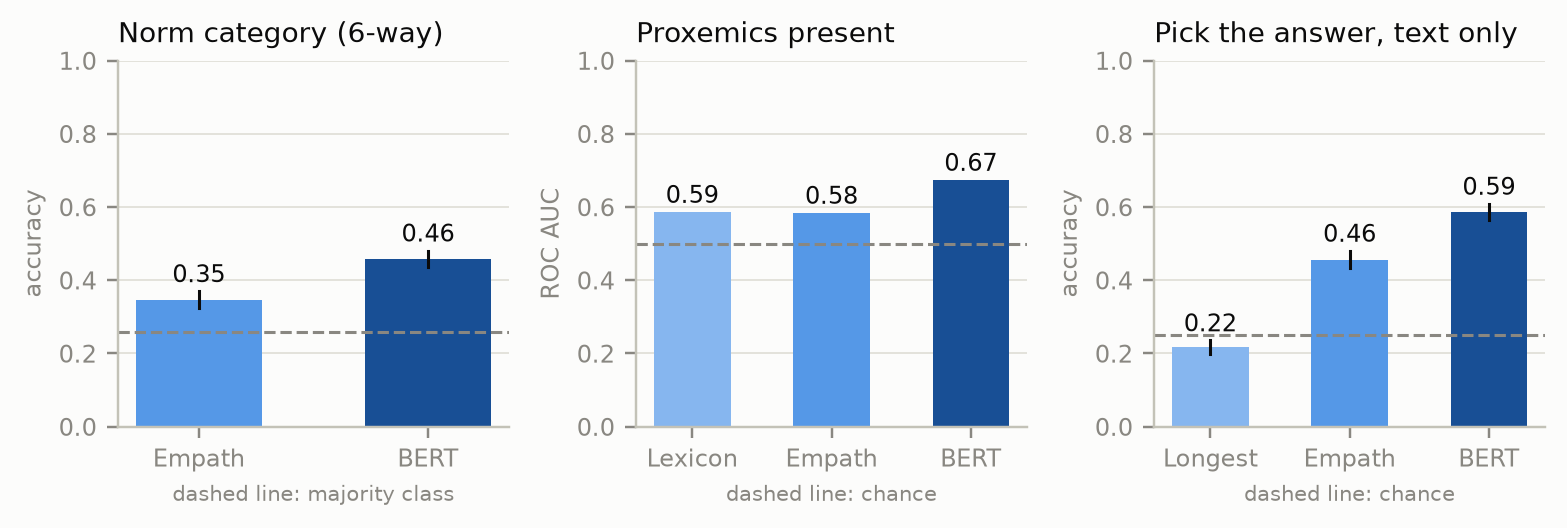
\includegraphics[width=\linewidth]{representation_comparison.png}
\caption{What each language representation recovers. Probes are cross-validated with folds grouped by source video; bars show 95\% bootstrap intervals where available.}\label{fig:lang-probe}
\end{figure}
\begin{figure}[t]\centering
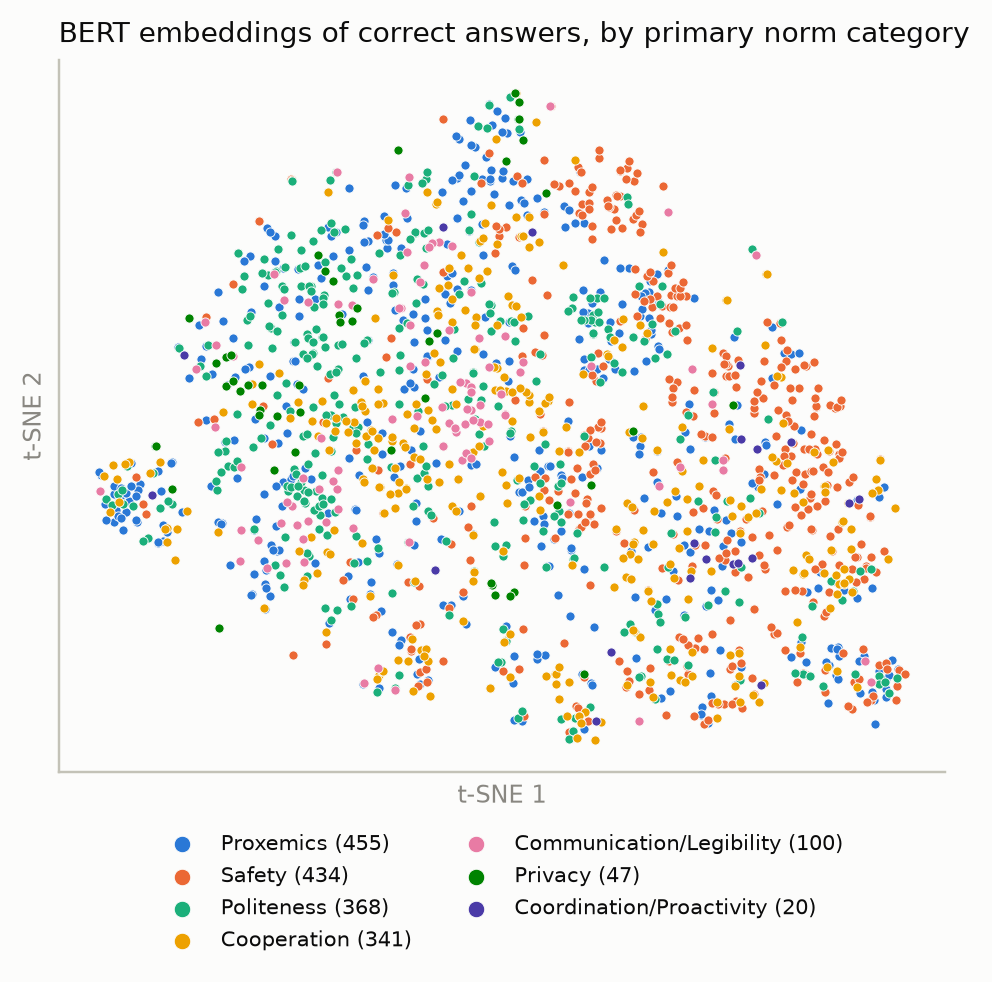
\includegraphics[width=0.9\linewidth]{tsne_category.png}
\caption{t-SNE of BERT embeddings of correct answer options, coloured by primary norm category.}\label{fig:lang-tsne}
\end{figure}
\begin{figure}[t]\centering
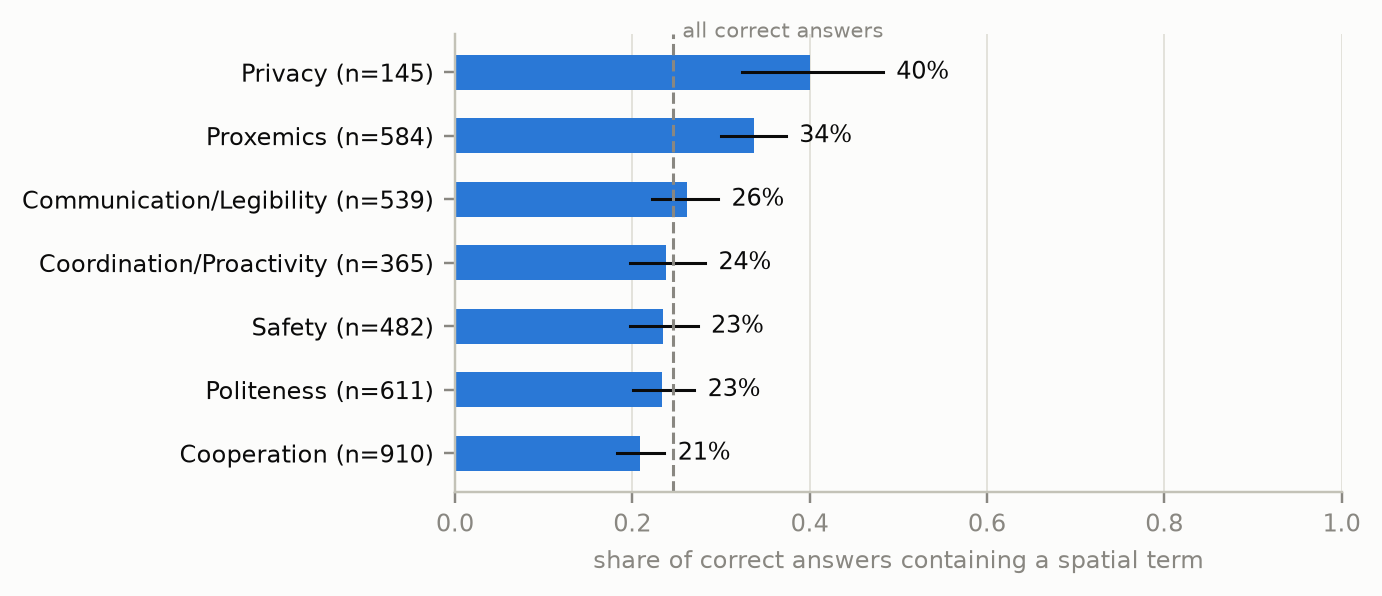
\includegraphics[width=0.9\linewidth]{spatial_language.png}
\caption{Share of correct options containing at least one spatial term, by norm category (an option can belong to several categories).}\label{fig:lang-spatial}
\end{figure}
\paragraph{Discussion of this analysis (provisional; author review required).} Three observations bear on idea 5. First, the option text leaks the label: a supervised text-only probe more than doubles chance without seeing the scene. The probe is trained on labelled items, so this is not a zero-shot score and is not comparable to leaderboard numbers, but it shows that correct options are written differently from distractors. Any gain attributed to geometry or pose must therefore be measured against a text-only baseline, not only against RGB. Second, spatial vocabulary is a minority signal: three in four correct answers contain no spatial term, and even within Proxemics two in three do not. Geometry is plausibly relevant to a subset of the benchmark rather than to all of it, which is consistent with our frozen-model analysis, where added maps changed almost no answers. This argues for evaluating idea 5 on the Proxemics and Privacy subsets separately instead of only on overall accuracy. Third, the contextual representation is consistently more informative than the interpretable ones, but the lexicon and Empath agree on direction (movement, body), which gives a transparent way to select the spatially relevant subset. Limitations: lexicon matching is crude (e.g.\ \emph{way}, \emph{clear}, \emph{close} have non-spatial senses), category labels are multi-label and we use the first listed as primary, and option text describes the candidate actions, not what is visible in the video.

% AI DISCLOSURE: Claude (Claude Code) wrote and ran scripts/language_exploration.py, produced the figures and numbers, and drafted this section. BERT and Empath produced the representations. Student review and interpretation are pending.
